Las misiones (\textit{Quests}) son uno de los pilares del género \textit{MMO RPG}. Gran parte de la experiencia 
de juego gira en torno a ellas, ya que constituyen el principal motor de progresión del jugador dentro del mundo. 
Juegos icónicos del género, como \textit{World of Warcraft} o \textit{RuneScape}, deben buena parte de su identidad 
precisamente a sus sistemas de misiones, que guían al jugador, le proponen objetivos concretos y lo recompensan 
por explorar el mundo.

\vspace{0.25cm}

En esta sección se describen las soluciones implementadas para la gestión de diálogos y misiones, comenzando por 
cómo un creador puede implementarlas en su mundo y, luego, cómo se presentan a los jugadores dentro del juego.

\subsubsection{Diálogos}
Los diálogos son la forma principal de interacción entre los jugadores y los \textit{NPCs} pasivos del juego, 
y son el medio a través del cual se presentan las misiones.

Cada diálogo está compuesto por una serie de mensajes que se muestran al jugador en orden secuencial, y cada 
mensaje contiene texto. Luego, en el editor de \textit{NPCs} pasivos, se puede asignar un diálogo a un \textit{NPC} 
y configurar si el diálogo agregado queda asociado a una misión.

\begin{figure}[H]
    \centering
    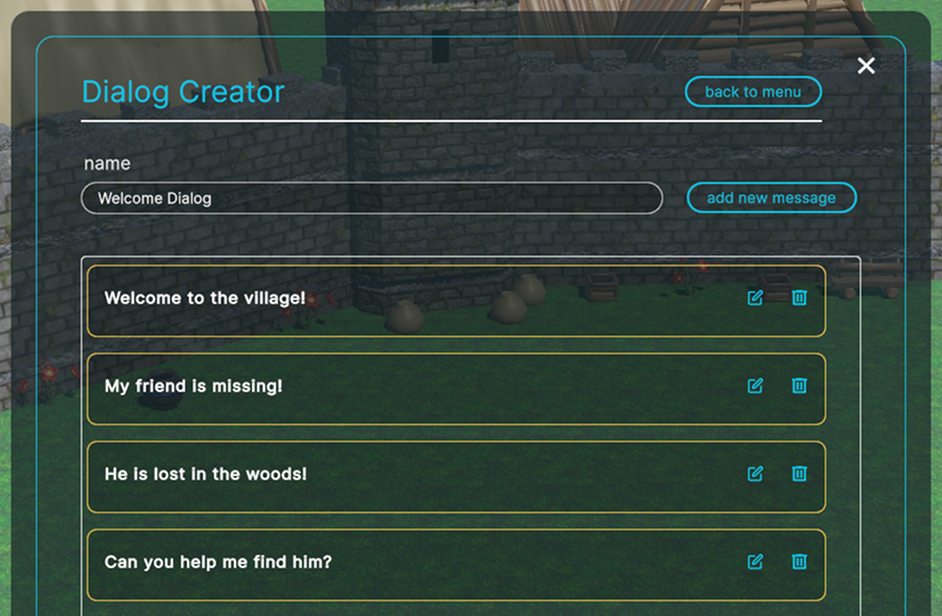
\includegraphics[width=0.6\textwidth]{img/08-implemented-solution/product/dialog-creation.jpg}
    \caption{Captura de pantalla del creador de diálogos.}
    \label{fig:dialog-creation}
\end{figure}

\subsubsection{Misiones}
Las misiones son tareas que los jugadores pueden aceptar y completar dentro del juego. Por el momento se ofrecen 
solo dos tipos de objetivos: matar un número específico de enemigos o interactuar con otro \textit{NPC} específico, 
aunque el sistema de misiones está diseñado para ser flexible y permitir la incorporación de nuevos tipos de objetivos 
en el futuro. El creador puede configurar las recompensas que el jugador recibirá al completarla: un valor en monedas 
de oro, ítems específicos o directamente un \textit{loot table} creado previamente, lo que permite una gran variedad 
de opciones.

\begin{figure}[H]
    \centering
    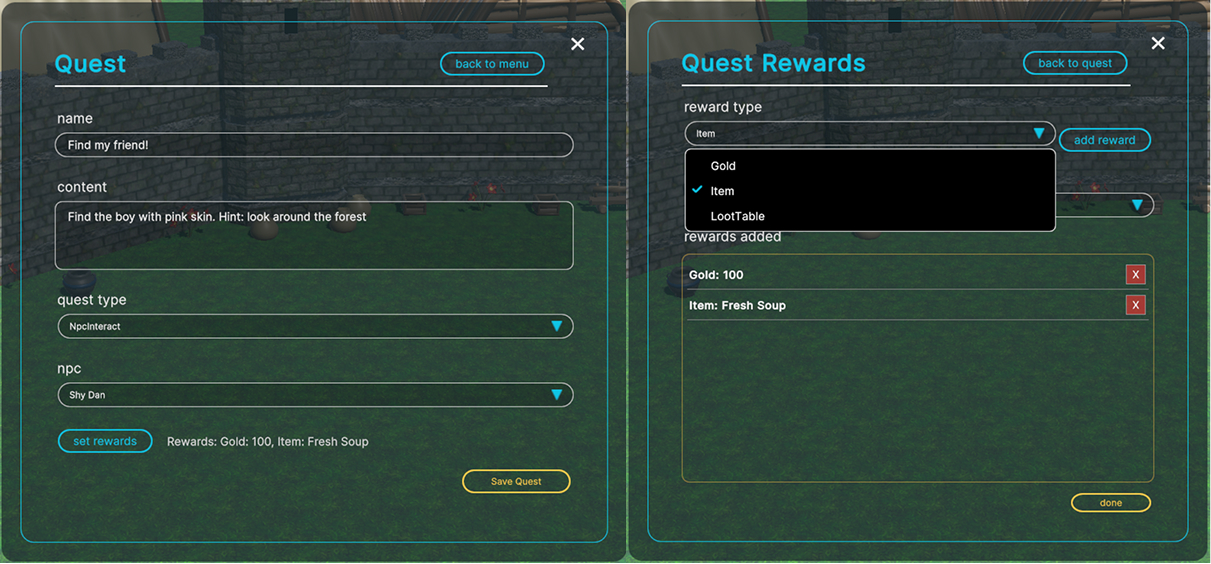
\includegraphics[width=1\textwidth]{img/08-implemented-solution/product/quest-creation.jpg}
    \caption{Captura de pantalla del creador de misiones.}
    \label{fig:quest-creation}
\end{figure}

Una vez creada una misión, el creador puede vincularla a un diálogo específico, de modo que el jugador pueda 
aceptarla o rechazarla al interactuar con el \textit{NPC} asociado a ese diálogo.

\subsubsection{Progresión de misiones}
Una funcionalidad interesante que se ha implementado es la posibilidad de crear una progresión de misiones a través 
de los diálogos. Esto se logra al permitir agregar nuevos diálogos contiguos a un mismo \textit{NPC} después de haber 
añadido una misión a uno de sus diálogos. De esta forma, el creador puede diseñar una experiencia de juego más compleja 
y ramificada, en la que los jugadores desbloquean nuevas misiones a medida que avanzan en la narrativa, e introducir 
además una progresión de dificultad en su mundo. También se puede configurar la repetibilidad de una misión, es decir, 
su capacidad de ser rehecha múltiples veces, lo que permite a los creadores diseñar misiones que los jugadores 
pueden completar varias veces para obtener recompensas adicionales, o misiones de una sola vez, que conservan su 
exclusividad y valor dentro del juego.

\begin{figure}[H]
    \centering
    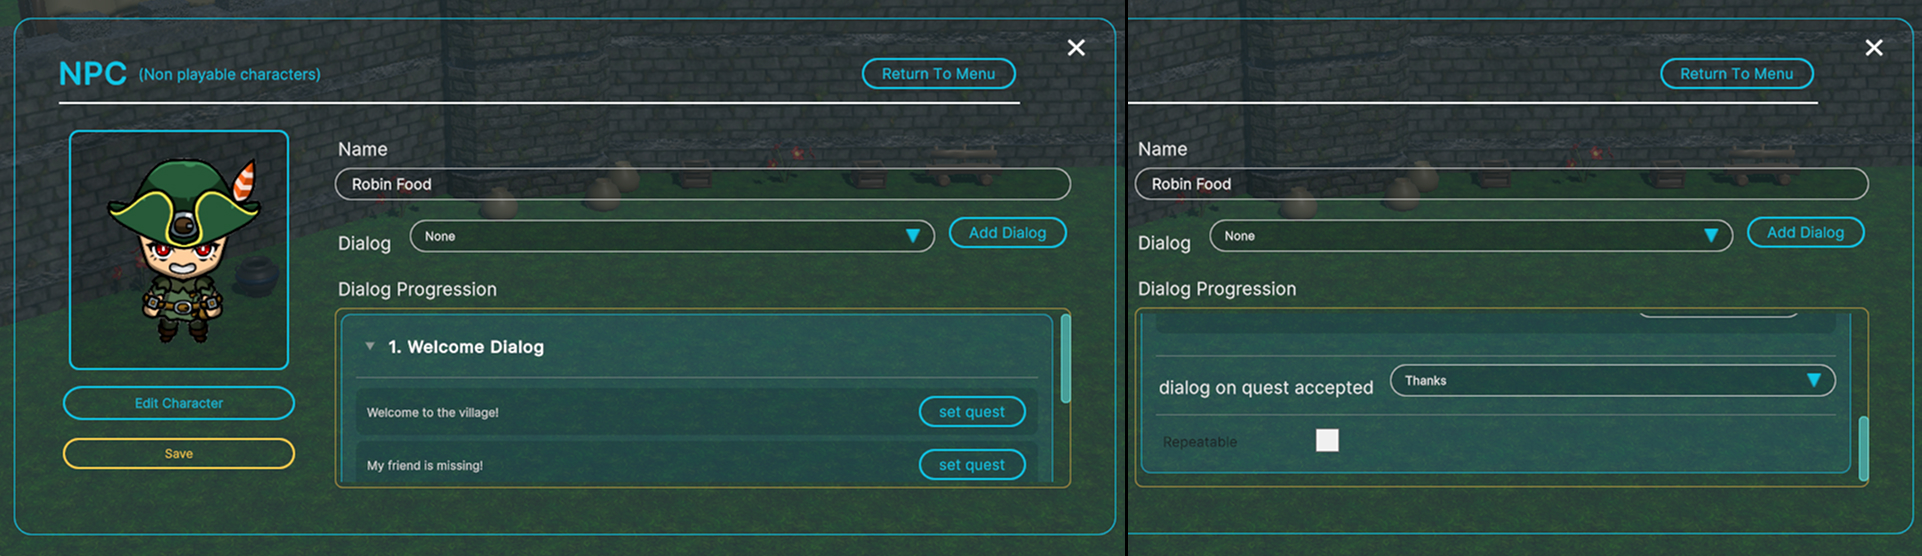
\includegraphics[width=1\textwidth]{img/08-implemented-solution/product/quest-npc.jpg}
    \caption{Captura de pantalla de un \textit{NPC} con una misión asignada.}
    \label{fig:quest-npc}
\end{figure}

\begin{figure}[H]
    \centering
    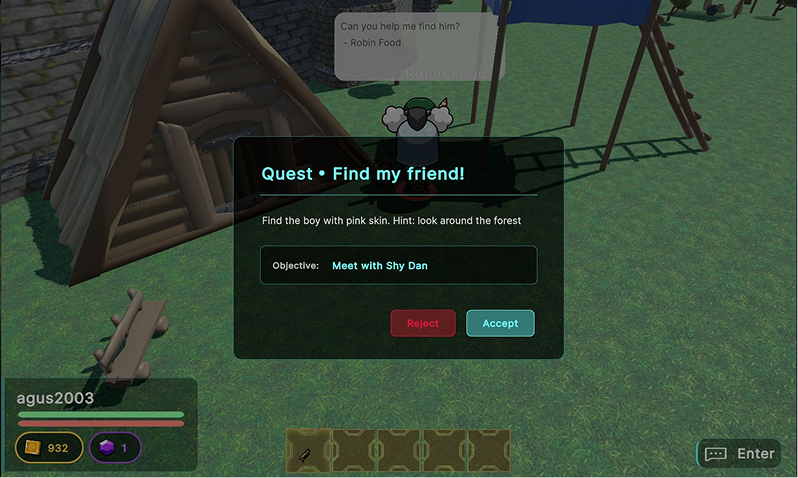
\includegraphics[width=0.70\textwidth]{img/08-implemented-solution/product/quest-accept.jpg}
    \caption{Captura de pantalla de un jugador aceptando una misión.}
    \label{fig:quest-accept}
\end{figure}

Cuando un jugador acepta una misión, esta se agrega a su lista de misiones activas y su progreso se muestra en pantalla. 
El jugador puede revisar los detalles de la misión en cualquier momento a través del menú de misiones.

\begin{figure}[H]
    \centering
    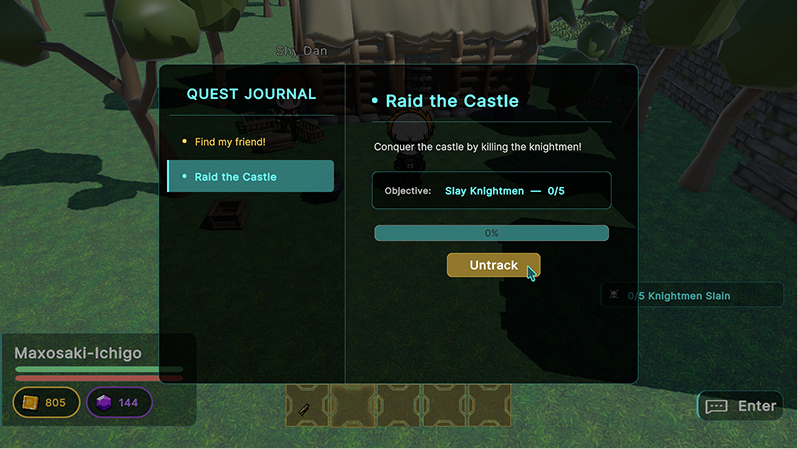
\includegraphics[width=0.85\textwidth]{img/08-implemented-solution/product/quest-journal.jpg}
    \caption{Captura de pantalla del diario de misiones.}    \label{fig:quest-journal}
\end{figure}

Al alcanzar el objetivo, la misión se completa automáticamente y el jugador recibe las recompensas configuradas. 
Como se mencionó previamente, si el creador dispuso más diálogos después de la misión, el jugador puede seguir 
interactuando con el \textit{NPC} para avanzar en la progresión.

\begin{figure}[H]
    \centering
    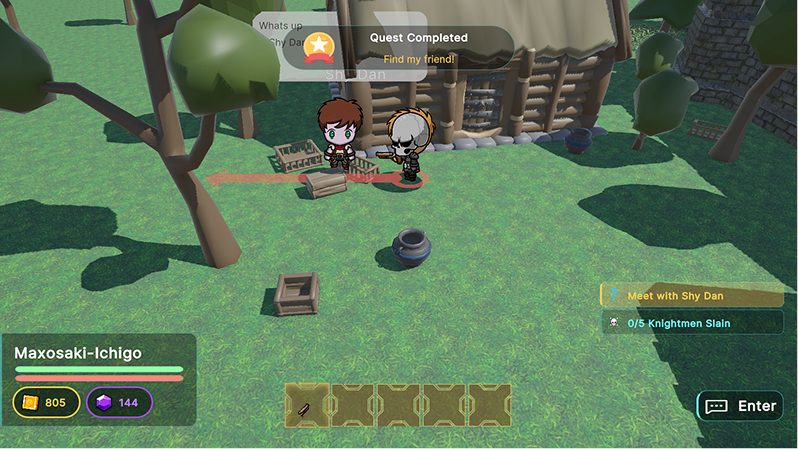
\includegraphics[width=0.85\textwidth]{img/08-implemented-solution/product/quest-completed.jpg}
    \caption{Captura de pantalla de un jugador completando una misión.}
    \label{fig:quest-completed}
\end{figure}

